% =====================================================================
% Diagrama de atividades do Louvain --- Arthur (Frente 4)
% Só o Arthur edita este arquivo. Salve a imagem em figuras/ e o código-fonte
% (PlantUML) em documentos/uml/.
% =====================================================================
\section{Diagrama de atividades do Louvain}\label{sec:atividades}

O algoritmo de Louvain~\cite{blondel2008} é um método heurístico eficiente para detecção de
 comunidades em redes complexas por meio da maximização da modularidade ($Q$). 
 A Figura~\ref{fig:atividades} apresenta o diagrama de atividades do algoritmo, 
 que opera em duas fases interdependentes executadas iterativamente até a convergência global.

Na \textbf{Fase 1 (Otimização Local)}, cada vértice inicia em sua própria comunidade individual. 
Os nós são visitados em ordem pseudo-aleatória 
(determinada por uma semente fixa para garantir reprodutibilidade). 
Para cada nó $v$, avalia-se o ganho de modularidade ($\Delta Q$) resultante de sua remoção 
da comunidade atual e inserção na comunidade de cada um de seus vizinhos. 
Se houver ganho estritamente positivo ($\Delta Q > 0$), o nó é transferido para a 
comunidade que proporcionar o maior aumento; caso contrário, ele permanece em sua posição original. 
Esse processo é repetido sequencialmente sobre todos os vértices até que nenhum nó mude de comunidade, 
alcançando um ótimo local.

Na \textbf{Fase 2 (Agregação da Rede)}, constrói-se um novo grafo ponderado reduzido, 
no qual cada comunidade obtida na primeira fase é colapsada em um único supernó. 
As arestas internas entre membros da mesma comunidade convertem-se em laços (\emph{self-loops}) 
com pesos somados, enquanto as conexões entre comunidades distintas tornam-se arestas ponderadas 
entre os respectivos supernós. 

O laço externo repete a Fase 1 sobre o grafo agregado resultante. O algoritmo encerra 
sua execução quando a modularidade global da rede estabiliza ($\Delta Q \le 0$). 
Ao final, a estrutura hierárquica de supernós é desempacotada, retornando a partição mapeada para 
os identificadores originais dos vértices e a modularidade final alcançada.

\begin{figure}[htbp]
\centering
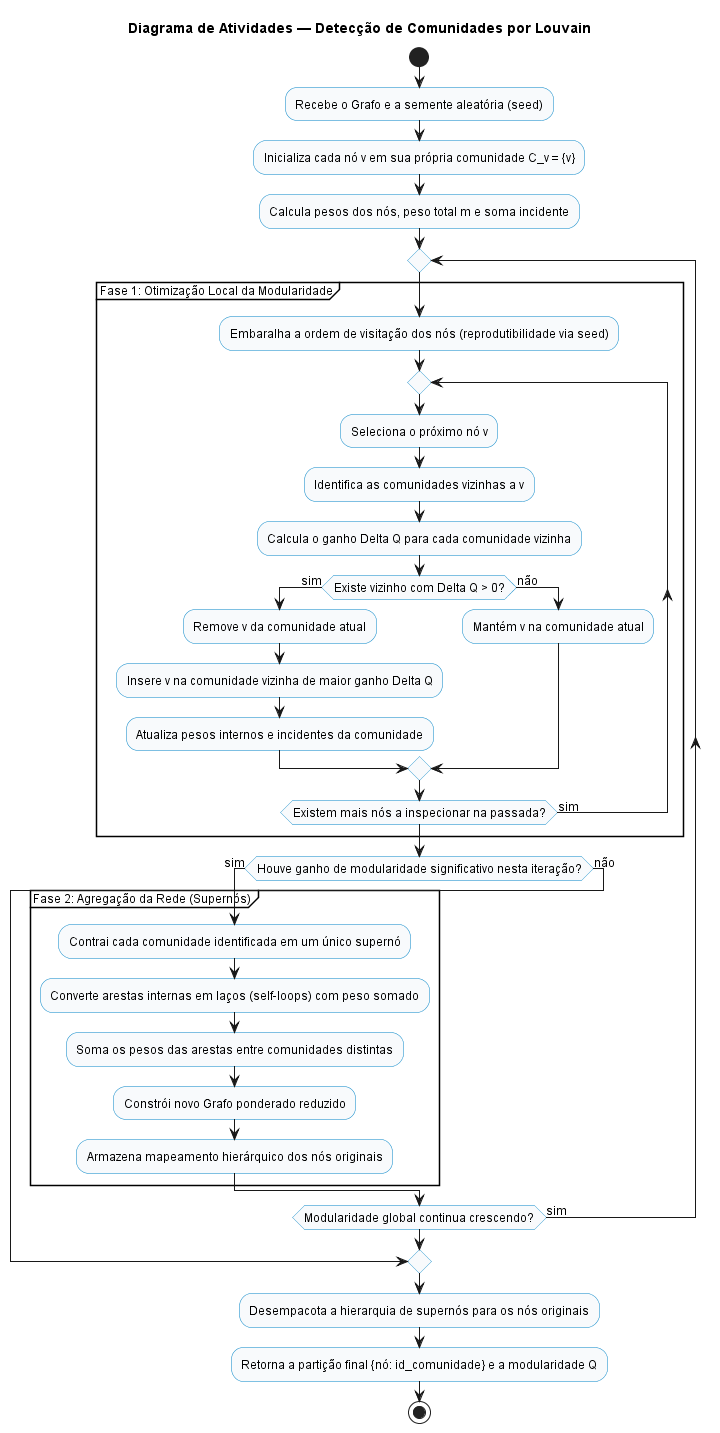
\includegraphics[width=.85\textwidth]{atividades_louvain.png}
\caption{Diagrama de atividades do algoritmo de Louvain.}
\label{fig:atividades}
\end{figure}
